\documentclass{article}
\usepackage{graphicx}
\graphicspath{ {graphs/} }
\usepackage{geometry}
\geometry{a4paper, portrait, margin=1.0in}
\usepackage{gensymb}
\usepackage{booktabs}
\begin{document}
\begin{titlepage}
    \begin{center}
        \vspace*{1cm}
        
        \Huge
        \textbf{Reconstruction of Charge Number of Heavy Cosmic Rays using Cherenkov Light}
        
        \LARGE
        
        \vspace{1cm}
        
        \textbf{Robert Stein}\\
        \textbf{CID 00819615}
        
        \vspace{1cm}
        
\includegraphics[width=0.4\textwidth]{Imperial_College_London_logo} 
        \hspace{0.5cm}
        
\includegraphics[width=0.4\textwidth]{hamburglogo}
        
        \vspace{1cm}
        
        Supervisor: Professor Dieter Horns
        
        \large
        \vspace{1.0cm}
        
        A thesis presented for the degree of\\
        \textbf{Master in Science}
        
        \vspace{0.5cm}

        Physics Department\\
        Imperial College London
        
        \vspace{0.5cm}
        
        \today
        
    \end{center}
\end{titlepage}
\section*{Abstract}
Between impact with the upper atmosphere and decay into a charged particle shower, heavy cosmic ray elements such as Iron emit Cherenkov Light at an angle determined by the Refractive Index of the air and the energy per nucleon. This direct Cherenkov Light forms a characteristic circular light distribution on the Earth's surface with an intensity proportional to the square of the cosmic ray charge. A new method has been developed to reconstruct this charge number, by fitting the received Cherenkov Photons to the characteristic Lateral Photon Distribution. The expected performance for various existing and planned installations will be discussed.

\section*{Zusammenfassung}
Between impact with the upper atmosphere and decay into a charged particle shower, heavy cosmic ray elements such as Iron emit Cherenkov Light at an angle determined by the Refractive Index of the air and the energy per nucleon. This direct Cherenkov Light forms a characteristic circular light distribution on the Earth's surface with an intensity proportional to the square of the cosmic ray charge. A new method has been developed to reconstruct this charge number, by fitting the received Cherenkov Photons to the characteristic Lateral Photon Distribution. The expected performance for various existing and planned installations will be discussed.
\newpage
\tableofcontents
\newpage

\section{Preface}
I basically just did everything. It was great.
\newpage

\section{Introduction}
There are numerous Telescope Arrays which image the Cherenkov Light emitted by Cosmic Rays in the atmosphere, including the HESS, MAGIC and VERITAS Experiments. All rely on Hillas Analysis with extracted parameters from each of the camera images being used to reconstruct the events, but heavy atmospheric blurring means that charge resolution is very poor. For Iron Nucleus events, we would expect to reconstruct \[Z \approx 26 \pm 5 \] with a core position resolution of roughly $d \approx 20 m $ \cite{hess07}. 

Cosmic Rays that are imaged by these telescopes have energies between $13 $TeV and $200 $TeV. At present, no study of the relative abundance of different cosmic ray elemental abundances exists at these energies. It could provide important clues regarding the mechanism of Cosmic Ray formation and propagation in the galaxy, but current charge resolution from Hillas Analysis is not small enough to undertake such a study.

Instead of Hillas Analysis, we consider a new method for event reconstruction, in which we fit the known Direct Cherenkovn (DC) Light observed by each telescope to a characteristic Lateral Photon Distribution (LPD) function. This new technique is valid both for currently running experiments, as well as planned experiments such as the Cherenkov Telescope Array (CTA). It uses only the information from the DC Pixel identified in the shower images.

A theoretical study by Kieda in 2001 \cite{kieda01} suggested that for a core position resolution of $d \approx 5 $ m, we could expect to see a charge resolution of $ \sigma_{Z} \approx 1 $ for elements of $Z = 20$ or higher. In this case the core position resolution would be the limiting value. Thus, if the LPD method can achieve this core position resolution, the precision will be sufficient to extract the abundances of the different Cosmic Ray Elements. This the prime motivation for the new LPD technique.

\section{DC Pixel Identification}
The first requirement for reconstruction using the LPD method is to identify the DC pixel in a shower image, and consequently determine the number of DC photoelectrons present. A full simulation of air showers was performed using the CORSIKA package, and the sim\textunderscore telarray package was used to simulate HESS camera images generated from the shower. A Boosted Decision Tree (BDT) was trained using image parameters to identify DC pixels, and its performance was tested. 

\subsection{CORSIKA}
A full simulation of Cosmic Ray air showers was performed using the CORSIKA package \cite{Heck98}, assuming a standard atmospheric profile derived from measurements conducted at the HESS site in Namibia. The simulated particles were $Fe^{56}$, within the Energy Range of $35-135$ TeV and a spectrum $\phi \propto E^{-2.7}$. For each set of simulated event, 4 unique random number seeds were used to generate the shower. An altitude of 1800m was assumed, again corresponding to the HESS site. The simulated zenith angle ranged from $0\degree < \theta < 2 \degree$, while the simulated azimuth angle ranges from $-2\degree < \phi < 2 \degree$. The four smaller HESS-phase-1 telescopes were arranged in a cross along the x/y axis with the larger HESS-phase-2 \textquoteleft CT5' telescope placed at the center. The length of each cross arm was $85m$. The simulated target region of the cores was chosen to be a square centered on CT5, with each 300m-long side bisecting the x/y axis.

In order to identify the DC pixel, a \textquoteleft DC Simulation' was initially run with an energy cut of 10 PeV on all muons and electrons. The consequence of this was to ensure that only the Cherenkov Light from the primary particle, as well as its fragments, was simulated. A second identical \textquoteleft Full Simulation' was run including the same random seeds, but without the energy cut on muons and electrons. This gave a complete air shower including the DC light, representative of those imaged in telescope arrays. Comparisons of the Full and DC simulations enabled us to identify background light in the Full shower.

\subsection{Sim\textunderscore telarray}
Using the sim\textunderscore telarray package \cite{Bernlohr08}, the expected hardware response to an air shower can be simulated. Again, the built-in response of the HESS telescope was selected for simulation. The program accounts for atmospheric transmission and density, mirror positions, sizes and reflectivities, camera shadowing and triggering, quantum efficiency and pulse responses. Due to the comprehensive and detailed nature of these hardware simulations, the resultant images can be considered representative of true camera images. For the Full Simulation, the night sky background was also simulated by sim\textunderscore telarray.

The HESS telescope has both a high gain Channel 0 and a low gain Channel 1. The location of each pixel (dependent on camera size), alongside the Sim\textunderscore telarray simulated value of SOMETHING? in each value was extracted. The pedestal and gain for each channel was also recorded, and from this, Intensity can be found.

\[ Intensity = (Count - Pedestal)\times Gain \]

In the case of many iron core events, Channel 0 will reach its maximum value and become saturated. Thus Channel 0 ceases to be useful for discriminating between high energy DC and non-DC pixels, so was not used in this analysis. Instead, only the Channel 1 was used in later analysis. Thus the Channel 1 Intensity will simply be referred to throughout this analysis as $Intensity$. 

In addition to the $Intensity$ of each pixel, the Sim\textunderscore telarray derives various Hillas whole-image parameters, which the script also extracted. These include the image width and length measured in degrees, from which the aspect ratio $A.R = \frac{width}{length}$ was calculated. Further the reconstructed shower direction and the shower center of gravity were calculated as positions in azimuth and zenith. Additionally the calculated energy and distance to core $r_{core}$ were recorded.

An entry was constructed for every pixel, containing its count and position. The variables $ \Delta_{C.o.G}$, $\Delta_{Direction}$ and $\Delta_{Line}$ were defined as the distance from the pixel to the shower center of gravity, shower direction, and the line joining those two points. Furthermore, the nearest neigbouring pixel IDs were calculated for every pixel position, enabling the count in each neighbouring pixel to be found. From this, two further pixel variables were defined. The largest neighbouring intensity $Intensity_{N.N.max}$ was found, and the ratio $ Q_{DC} = \frac{Intensity}{Intensity_{N.N.max}} $ was derived. In addition the Nearest Neighbour Mean Count was recorded. These variables were recorded in every pixel entry, and together the pixel entries formed a complete dataset for each camera image.

\subsection{Classic DC Identification}
The original method used by the HESS collaboration \cite{hess07} was initially replicated, for which a number of cuts were applied to each image dataset.

\begin{table}[h!]
  \centering
  \caption{Cuts applied to image pixel sets}
  \label{tab:table1}
  \begin{tabular}{ccc}
    \toprule
    Variable & Cut\\
    \midrule
     $r_{core}$ & \textgreater 0.4 \\
     $Q_{DC}$ & \textgreater 1.3 \\
     $ \Delta_{C.o.G}$ & \textgreater 0.17 \\
     $ \Delta_{C.o.G}$ & \textless 0.91 \\
     $\Delta_{Direction}$ & \textless 0.45 \\
     $\Delta_{Line}$ & \textless 0.23 \\
     Aspect Ratio & \textless 0.75 \\
    \bottomrule
  \end{tabular}
\end{table}

From the subset of pixels satisfying these conditions, the remaining pixel with the largest $Q_{DC}$ was selected as the DC pixel. The result was compared with the true DC pixel, identified from the hadron-only image, to test the accuracy of this cut. Out of 400 events, it was fount that only 55\% of these events contained a clear DC signal, as defined by requiring the DC pixel to have $Intensity_{DC} > 150$ in the hadron-only image. SOMETHING! Of this subset of 'DC events', 17\% events passed all of the required cuts. The $Q_{DC}$ was found to be 100\% accurate in identifying the DC pixel in those passing events, as shown in \ref{fig:cutdistribution}.

\begin{figure}
\begin{center}
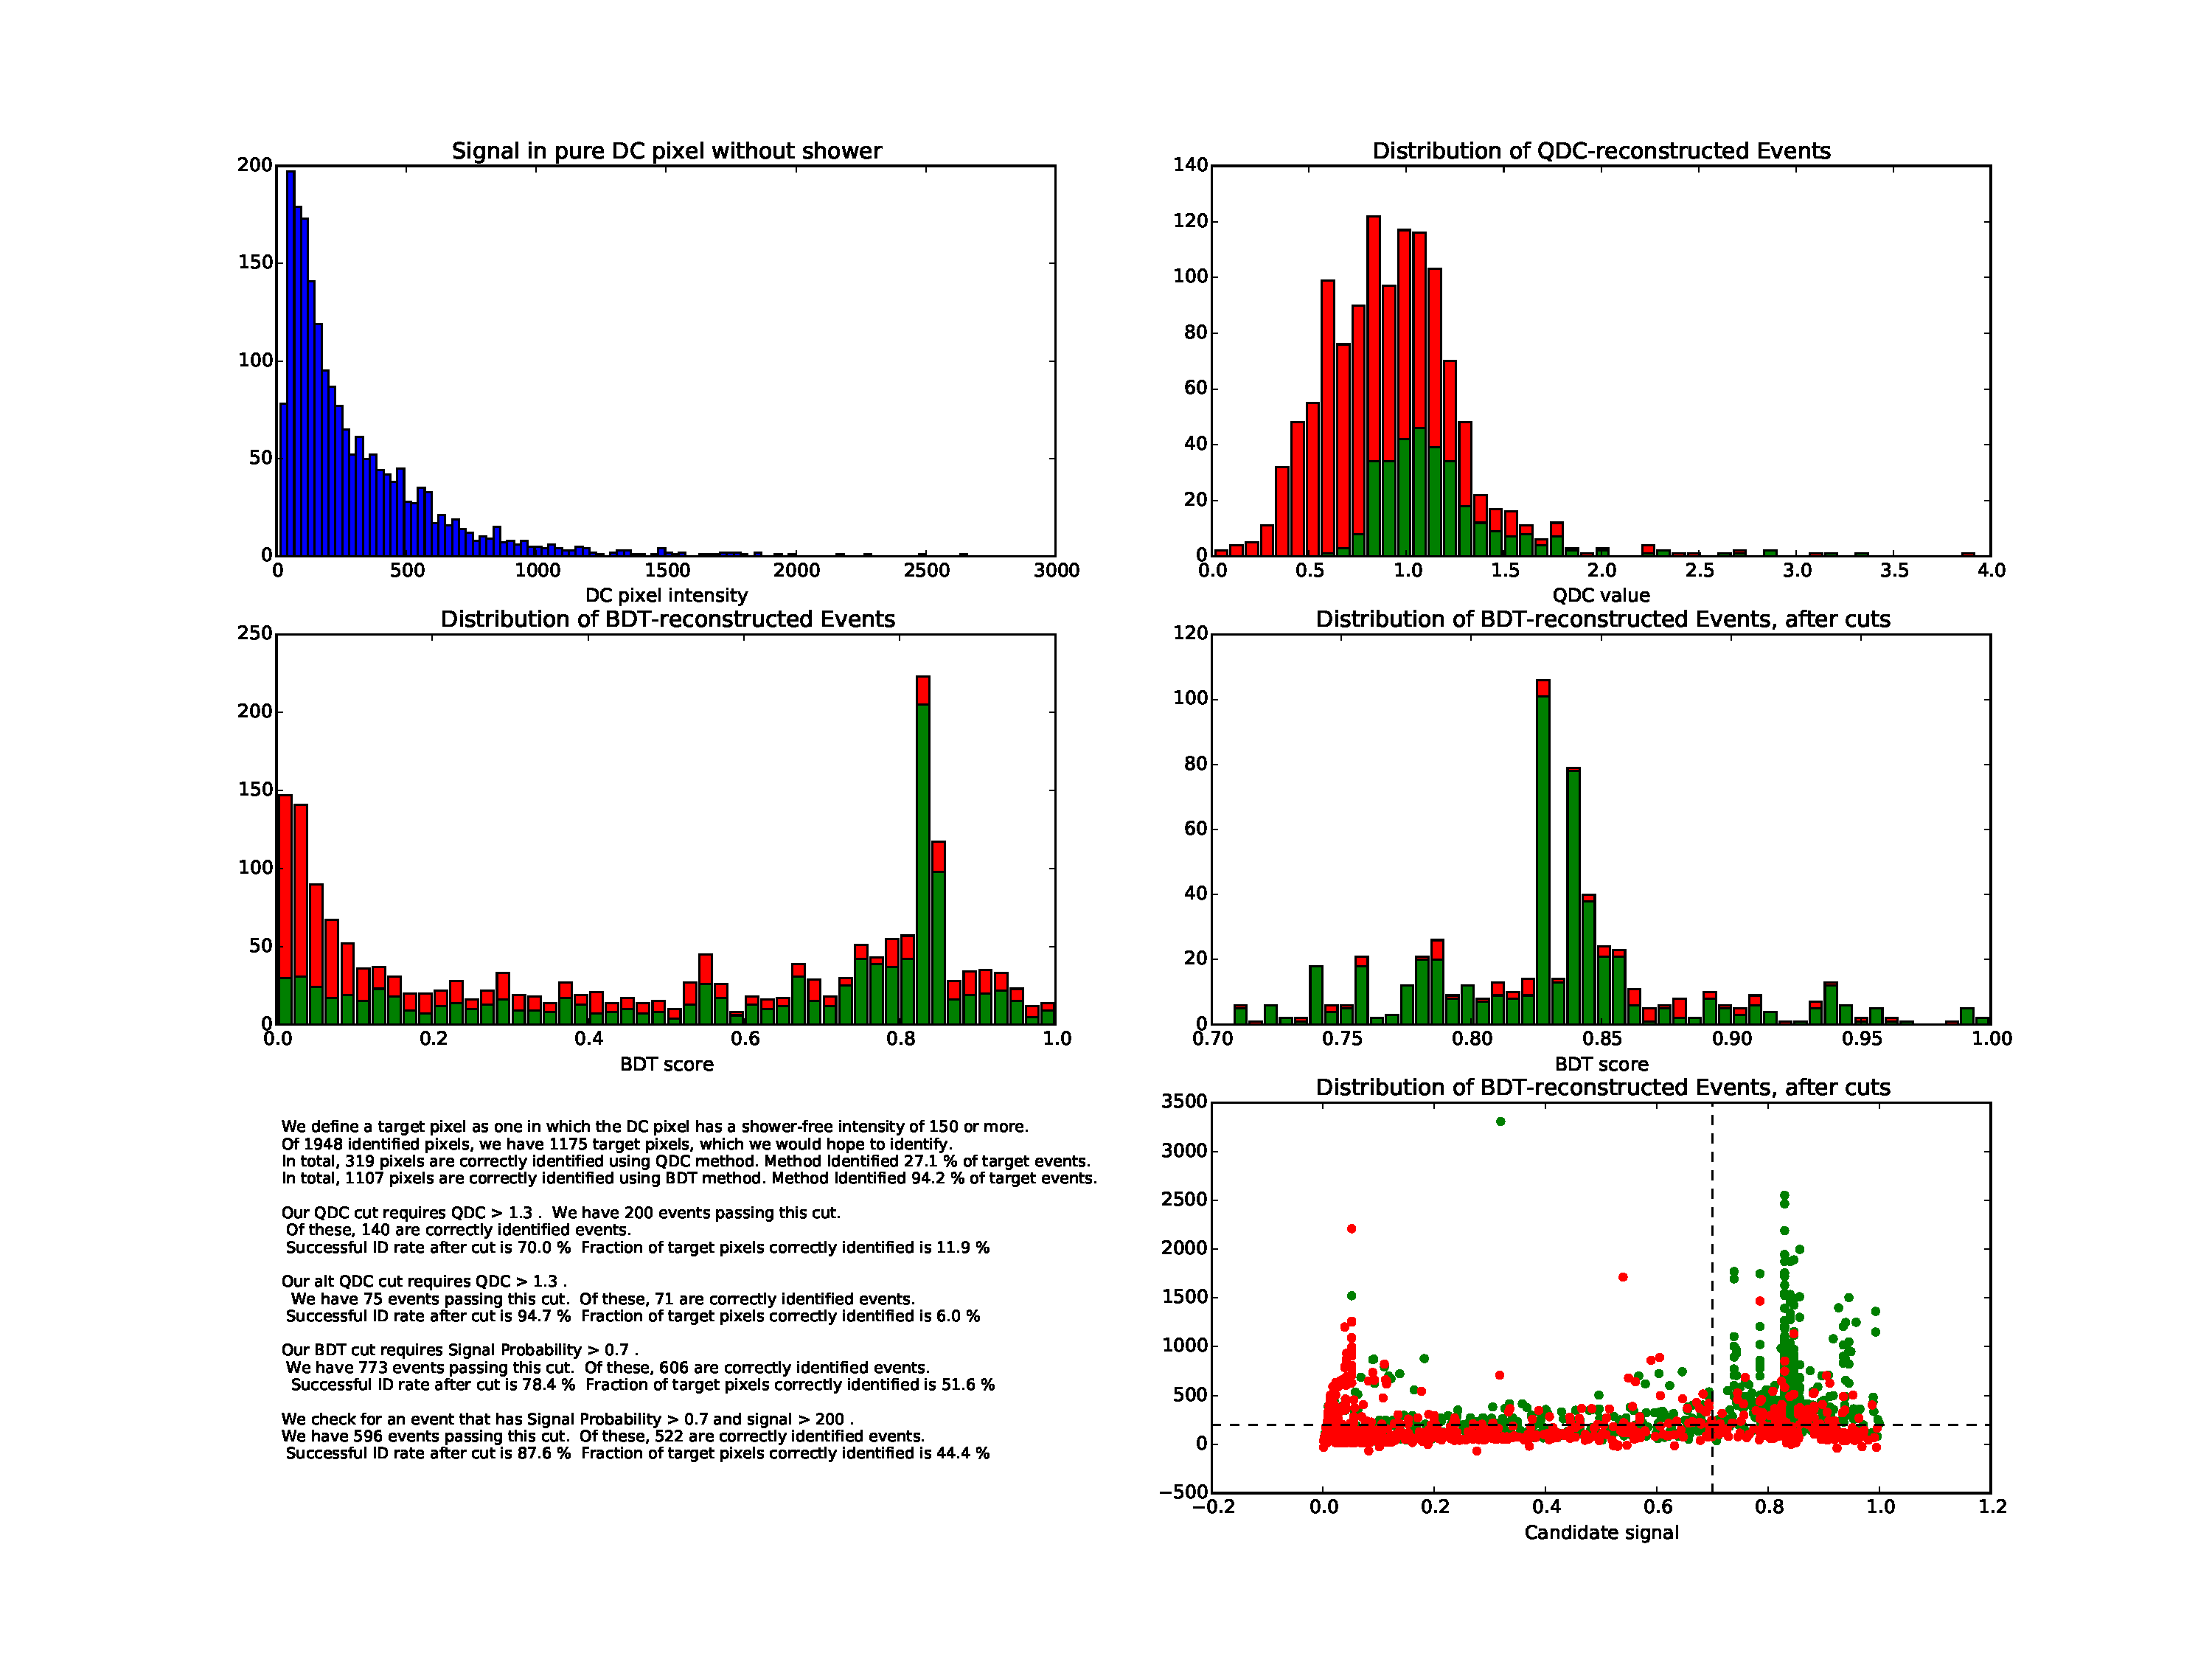
\includegraphics[width=\textwidth]{cutdistributionhess1}
\caption{The DC signal in the shower-free pixel is shown in the top left, with a broad gaussian distribution with the tail of the night-sky background extending up to appproximately 5000. Events below this are unlikely to be identified correctly because the DEC light is too faint. In the top right- the distribution of the dataset is shown, once all the non-$Q_{DC}$ cuts have been applied. In the bottom left, the BDT score distribution is shown before any cuts. On the bottom right, we see the same distribution after both signal and BDT score cuts are applied. All green events are ones in which the DC pixel has been correctly identified, while red events are ones that have been incorrectly identified.}
\label{fig:cutdistribution}
\end{center}
\end{figure} 

\subsection{Boosted Decision Tree DC Identification}  As an alternative to use of $Q_{DC}$, a new method of DC pixel identification was developed as part of this analysis by using a BDT trained with the Scikit Learn Python package. A set of 2000 simulated events was selected, and randomly split through use of the python random.random() function into two subsets for training and testing. The variable $DC_{Count} = Count-Mean_{N.N}$ was defined as an approximate \textquoteleft DC signal', if the pixel were to be selected as the DC candidate. For every pixel in the 2000 simulated events HESS 1 images, an entry was formed of $Q_{DC}$, $ \Delta_{C.o.G}$, $\Delta_{Direction}$, $\Delta_{Line}$, Channel1, Channel0, $DC_{Count}$ and $Mean_{N.N}$. A score of 0 was assigned to every pixel to indicate background, with the exception of those that were identified as the DC pixel through the Shower-Free simulation. If the DC count in the shower-free simulation was larger than 300, the pixel was included with a score of 1, identifying it as a signal pixel. Pure DC pixels below the threshold cut of 300 were deemed to be too faint to reconstruct, so these entries were omitted from the training set.

Having created a dataset, the BDT was then trained with a maximum depth of 5, and 100 trees generated. It was found that the BDT was 100 \% accurate for the entire training dataset, with a breakdown of 100 \% for the training background and 99 \% accurate with the training signal. When the trained BDT was applied to the testing pixels, it was found to be 99.99 \%  accurate for the entire training dataset, with a breakdown of 100 \% for the testing background and 99 \% accurate with the testing signal. This indicates that the BDT was not significantly overtrained, which would otherwise be manifested by a large divergence in accuracy between testing and training data.

\subsection{Composite Event Selection}
Having trained the BDT successfully, it was then applied to the same dataset as for the classic QDC identification. In each camera image, the event with the largest BDT score was deemed to be \textquoteleft most signal-like', and thus selected as the DC pixel candidate. A cut was applied, requiring $Probability_{signal} > 0.5$ for the DC candidate to be accepted. 

With this cut applied, out of 1200 events, 46\% events passed all of the required cuts. The BDT was found to be 75 \% accurate in identifying the DC pixel in those passing events.

In \ref{fig:cutdistribution}, a plot of true vs. reconstructed DC count is shown, obtained by comparing the BDT selected pixel to the hadron-only DC pixel. The black line indicates the optimal 1:1 ratio that we are aiming for. It is seen that there the vast majority of misidentified events have a small $candidate_{DC count}$, forming a red line in the region $candidate_{DC count} \approx 0$. To remove these misidentified events, we can apply a second cut requiring $candidate_{DC count} > 300$.

Application of this combined cut greatly increases the successful identification rate. Of the 2000 events, 84\% of events passed all of the required cuts. The BDT was found to be 90 \% accurate in identifying the DC pixel in those passing events. This represents a very significant improvement in DC pixel identification over the previous QDC method, and corresponds to a fivefold increase in the number of HESS data events that can be studied using the LPD method. Use of this BDT method is thus assumed throughout the rest of this analysis.

\subsection{Error in calculated $Count_{DC}$}
Having successfully identified the DC pixel in many events, we can calculate the difference between the derived $candidate_{DC count}$ and the hadron-only $True_{DC}$ to determine the error we will find for the LPD. Binning the difference $\Delta = candidate_{DC count} - True_{DC count}$ as shown in FIG, we find that the mean difference is 65 and the median difference is -75. We thus see that the distribution is not significantly skewed. However, the Standard deviation is approximately 600 when measured both by half of the difference from the 16th to 84th centile, and by 68th centile of an absolute difference. This again suggests that, although skewed, the fraction error in intensity is rather large. However, the fractional error found purely on the basis of QDC calculations is EQUALLY LARGE??LARGER?.

\begin{figure}
\begin{center}
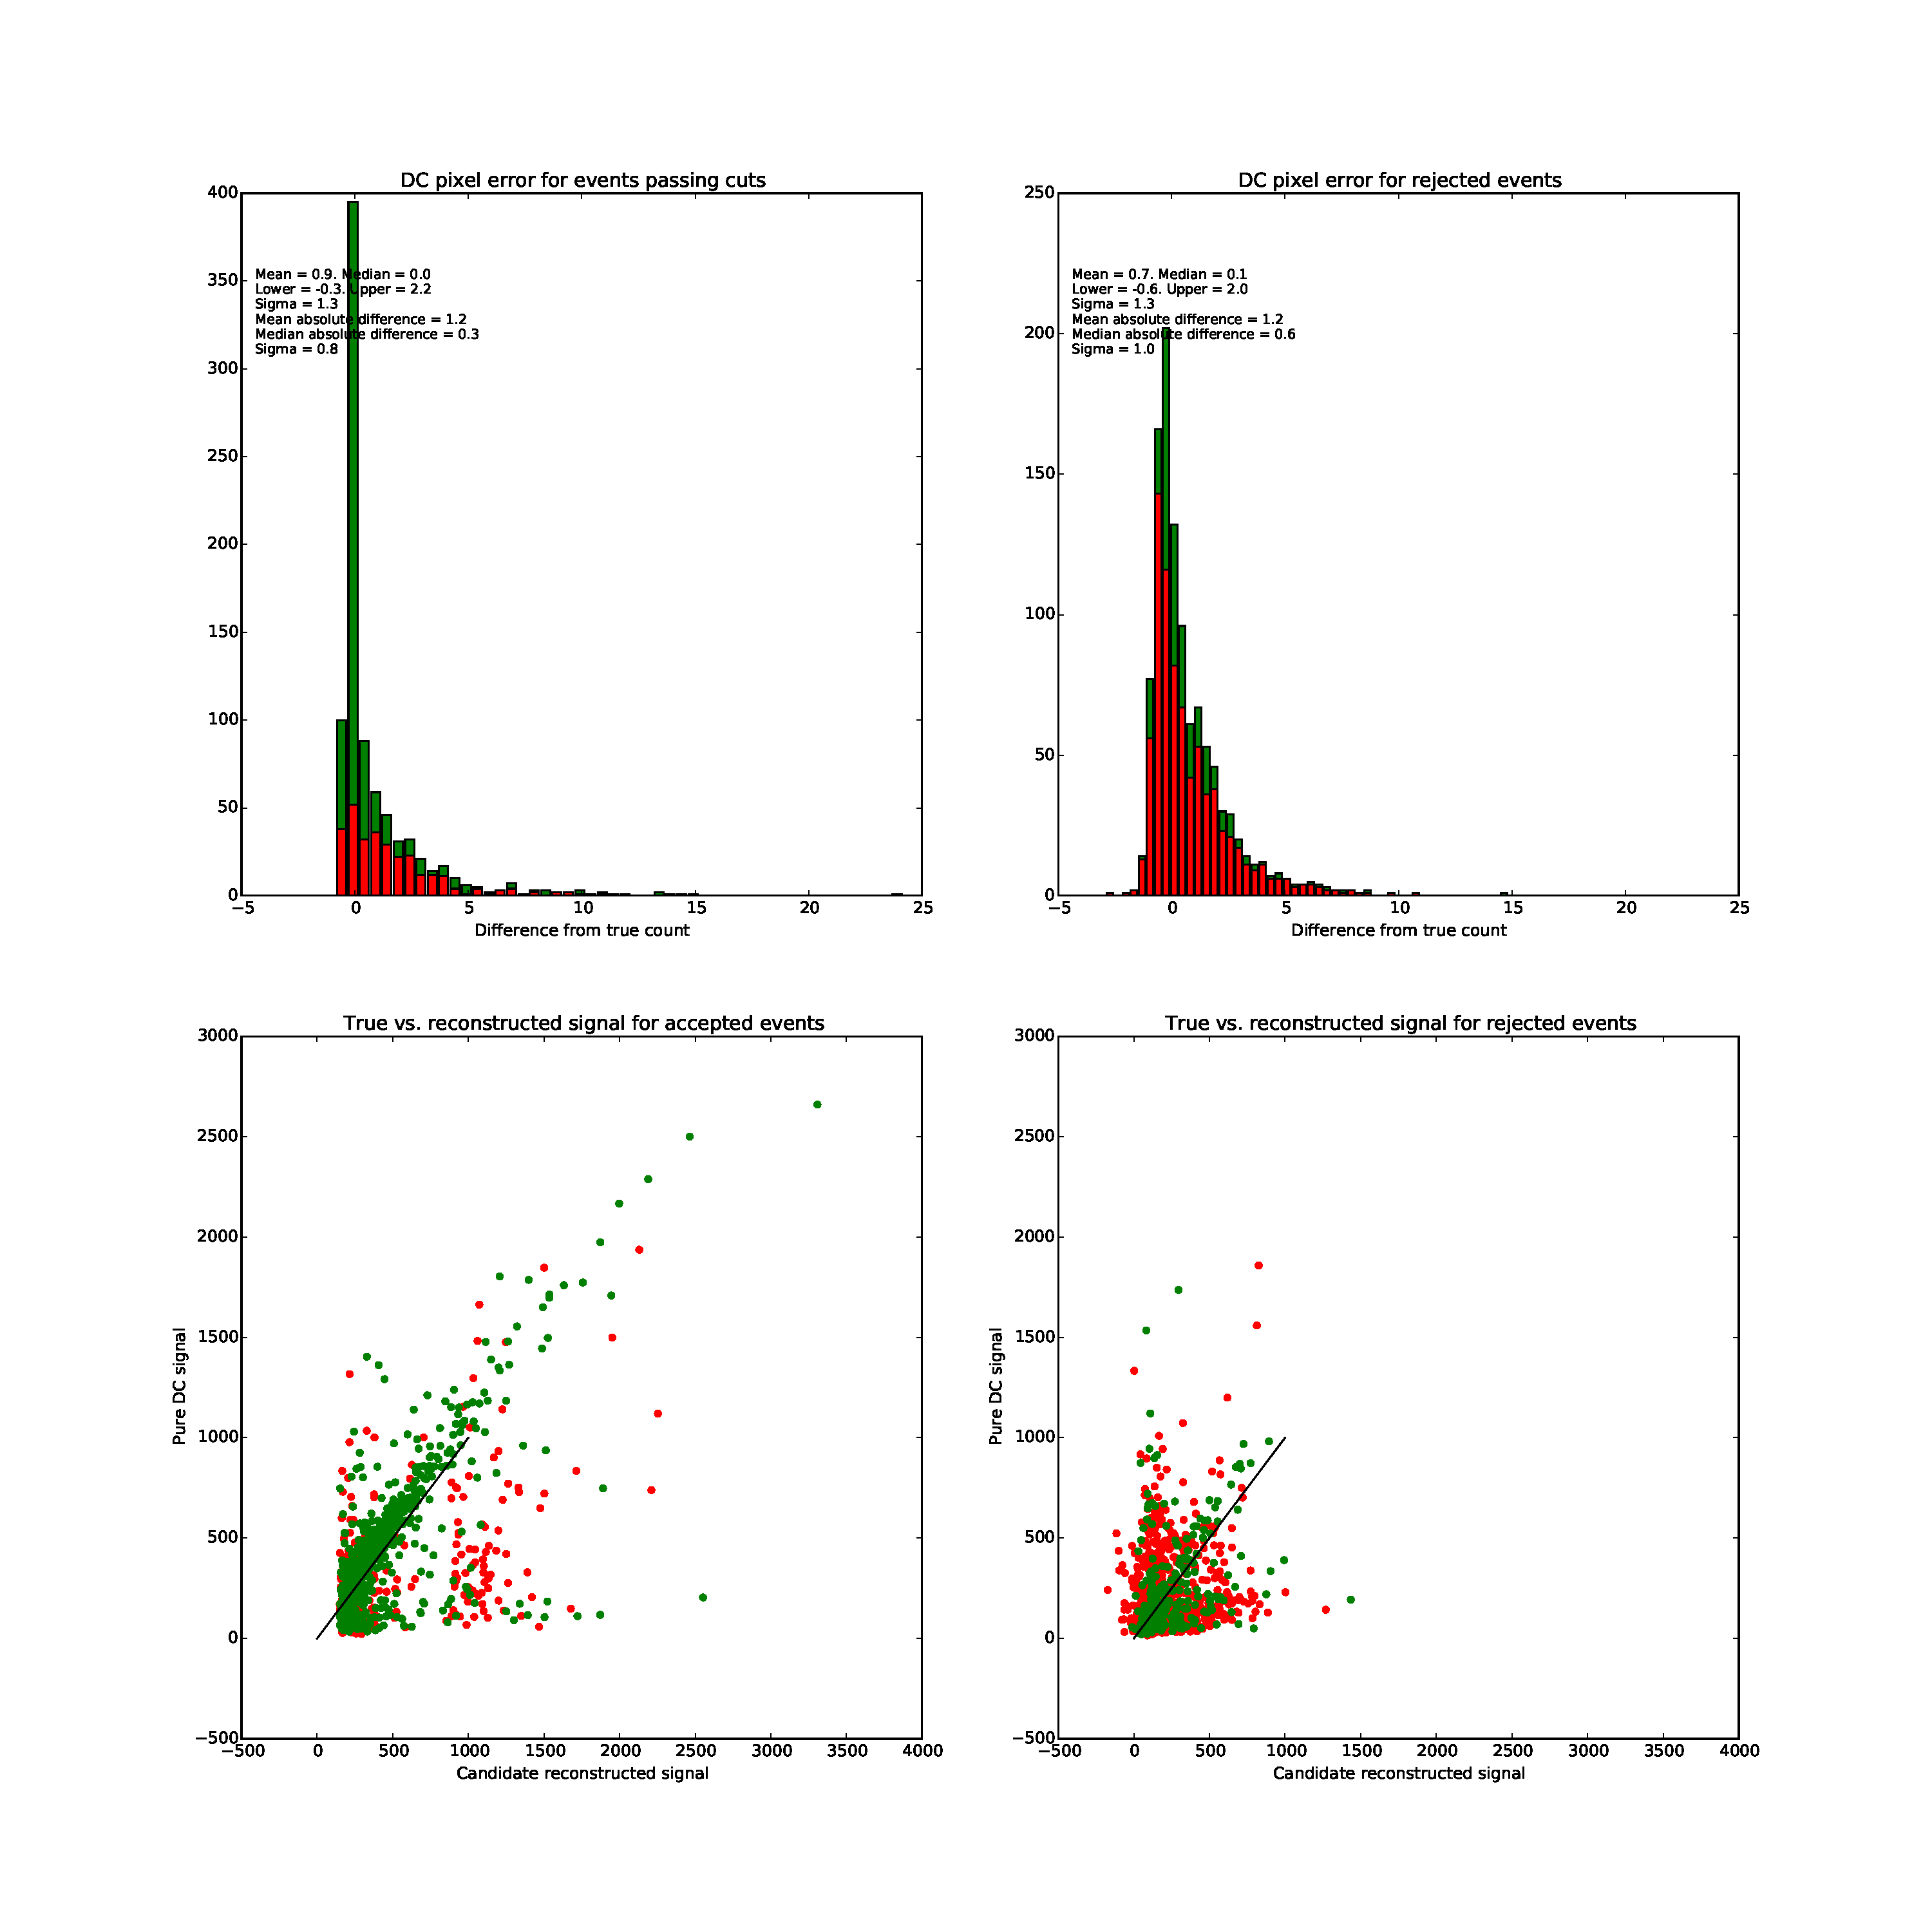
\includegraphics[width=\textwidth]{DCcounterrorhess1}
\caption{The difference between true and reconstructed DC signal for events passing the cuts is shown in the top left. In the top right the same is shown for events which were rejected. The true DC signals for events which passed the cuts is plotted against the reconstructed signals in the lower left, and for rejected events in the lower right. As in \ref{fig:cutdistribution}, in all plots a green event is one in which the DC pixel has been correctly identified, while a red event is one that has been incorrectly identified.}
\label{fig:dcdiff}
\end{center}
\end{figure}

\section{Cosmic Ray Event Simulation}
In order to reconstruct events using the LPD method, we require saturation of the Cosmic Ray Energy, and that the event can be seen by at least 4 telescopes. These restrictions confine us to Cosmic Rays with specific characteristics.

\subsection{Cherenkov Emission}
Cosmic Rays follow a well-defined power law where $ \frac{dN(E)}{dt} \propto E^{-\gamma} $ and experimentally $ \gamma = 2.7 \pm ? $. Consequently higher energy Cosmic Rays are heavily suppressed. The Energy Threshold for Cherenkov Light Emission as a function of height is illustrated in \ref{fig:generalenergy}. Once the Energy of a Cosmic Ray exceeds the local Cherenkov Energy Threshold of the atmosphere, the Nucleus will begin emitting a ring of Cherenkov Light. 

Above threshold, Cherenkov Emission is determined by the Frank Tamm formula!!!!! A full simulation of the LPD was undertaken. Under the assumption of constant magnetic permittivity and a zenith angle of $90\degree$ we can use the approximate form \[ N_{photons} \approx (37000 \times Z^{2} \times \Delta_{h} \times \Delta_{E})\] where $\Delta_{h}$ is the vertical distance travelled in meters and $\Delta_{E}$ is the emission energy range in eV.

If we divide the number of emitted photons by the area of the annulus between the ring radii at $h$ and $h - \Delta_{h}$, we retrieve the LDF shown in \ref{fig:lpd}, which varies with $ \rho_{DC}  = f(r) \times Z^{2}$ . Thus the amplitude of the LDF is proportional to the charge of the Cosmic Ray, enabling the Charge to be determined from the DC emission. This is the basis for charge reconstruction in the LDF method.

\begin{figure}
\begin{center}
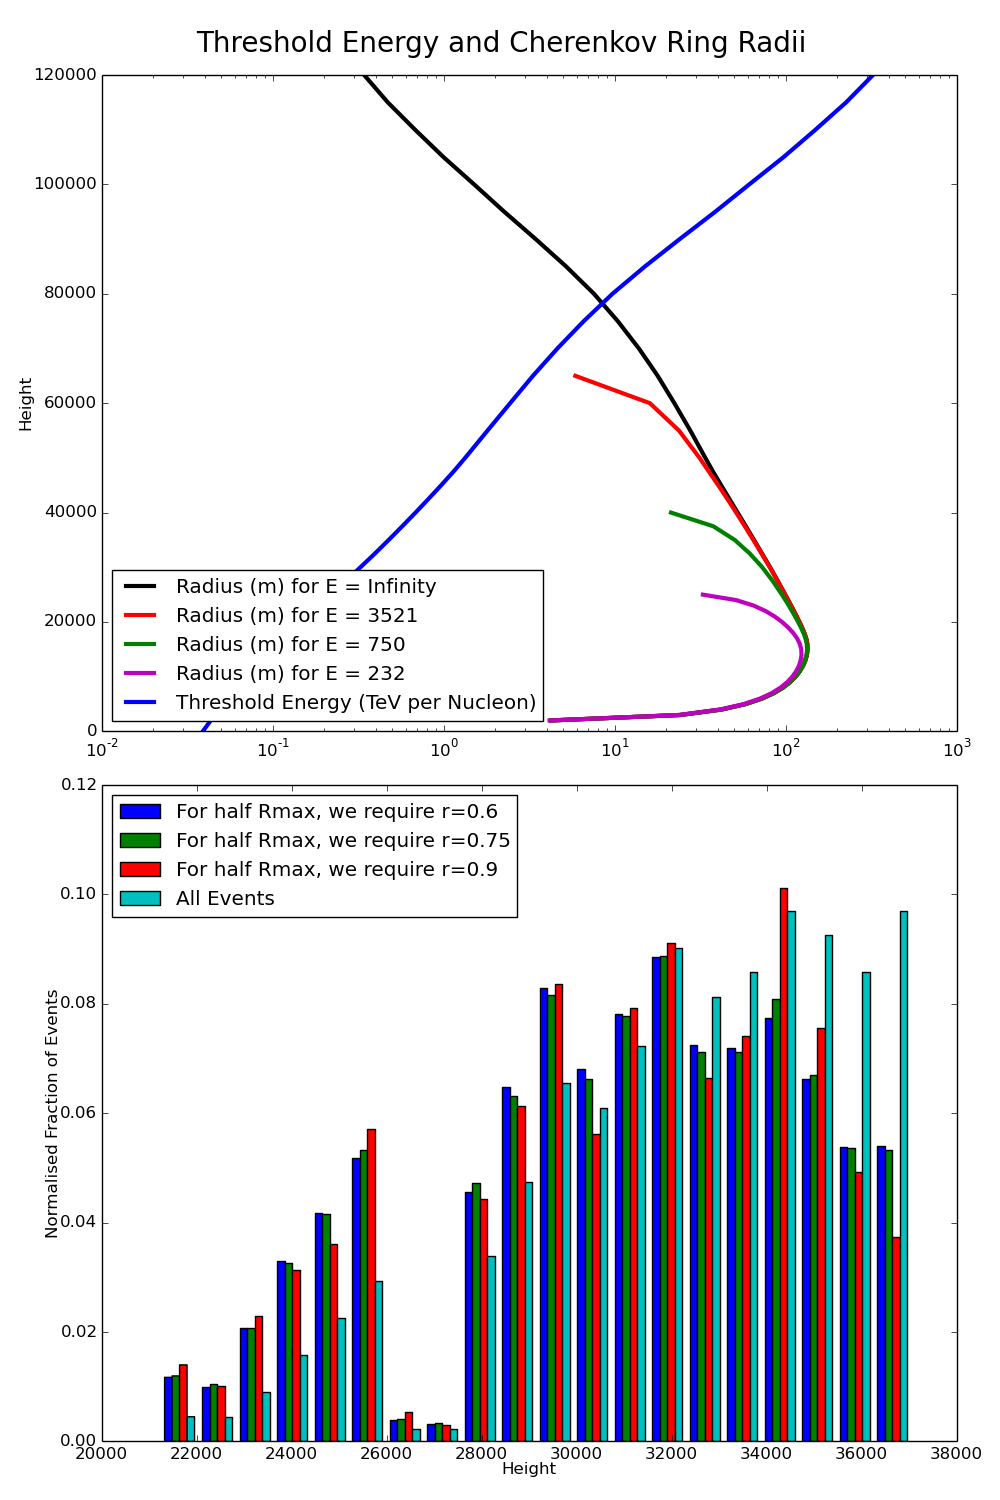
\includegraphics[height=0.9\textheight]{logenergyradius}
\caption{The Threshold Energy for Cherenkov Emission is marked in blue. With the assumption of $\beta=1$, the maximum emission radius is marked in black. The red and green and magenta line show the emission radius at 3.57 and 0.75 and 0.23 TeV per Nucleon respectively. The Green line is sufficiently close to the background to be saturated at 24km, while the magenta line is not.}
\label{fig:generalenergy}
\end{center}
\end{figure}

\begin{figure}
\begin{center}
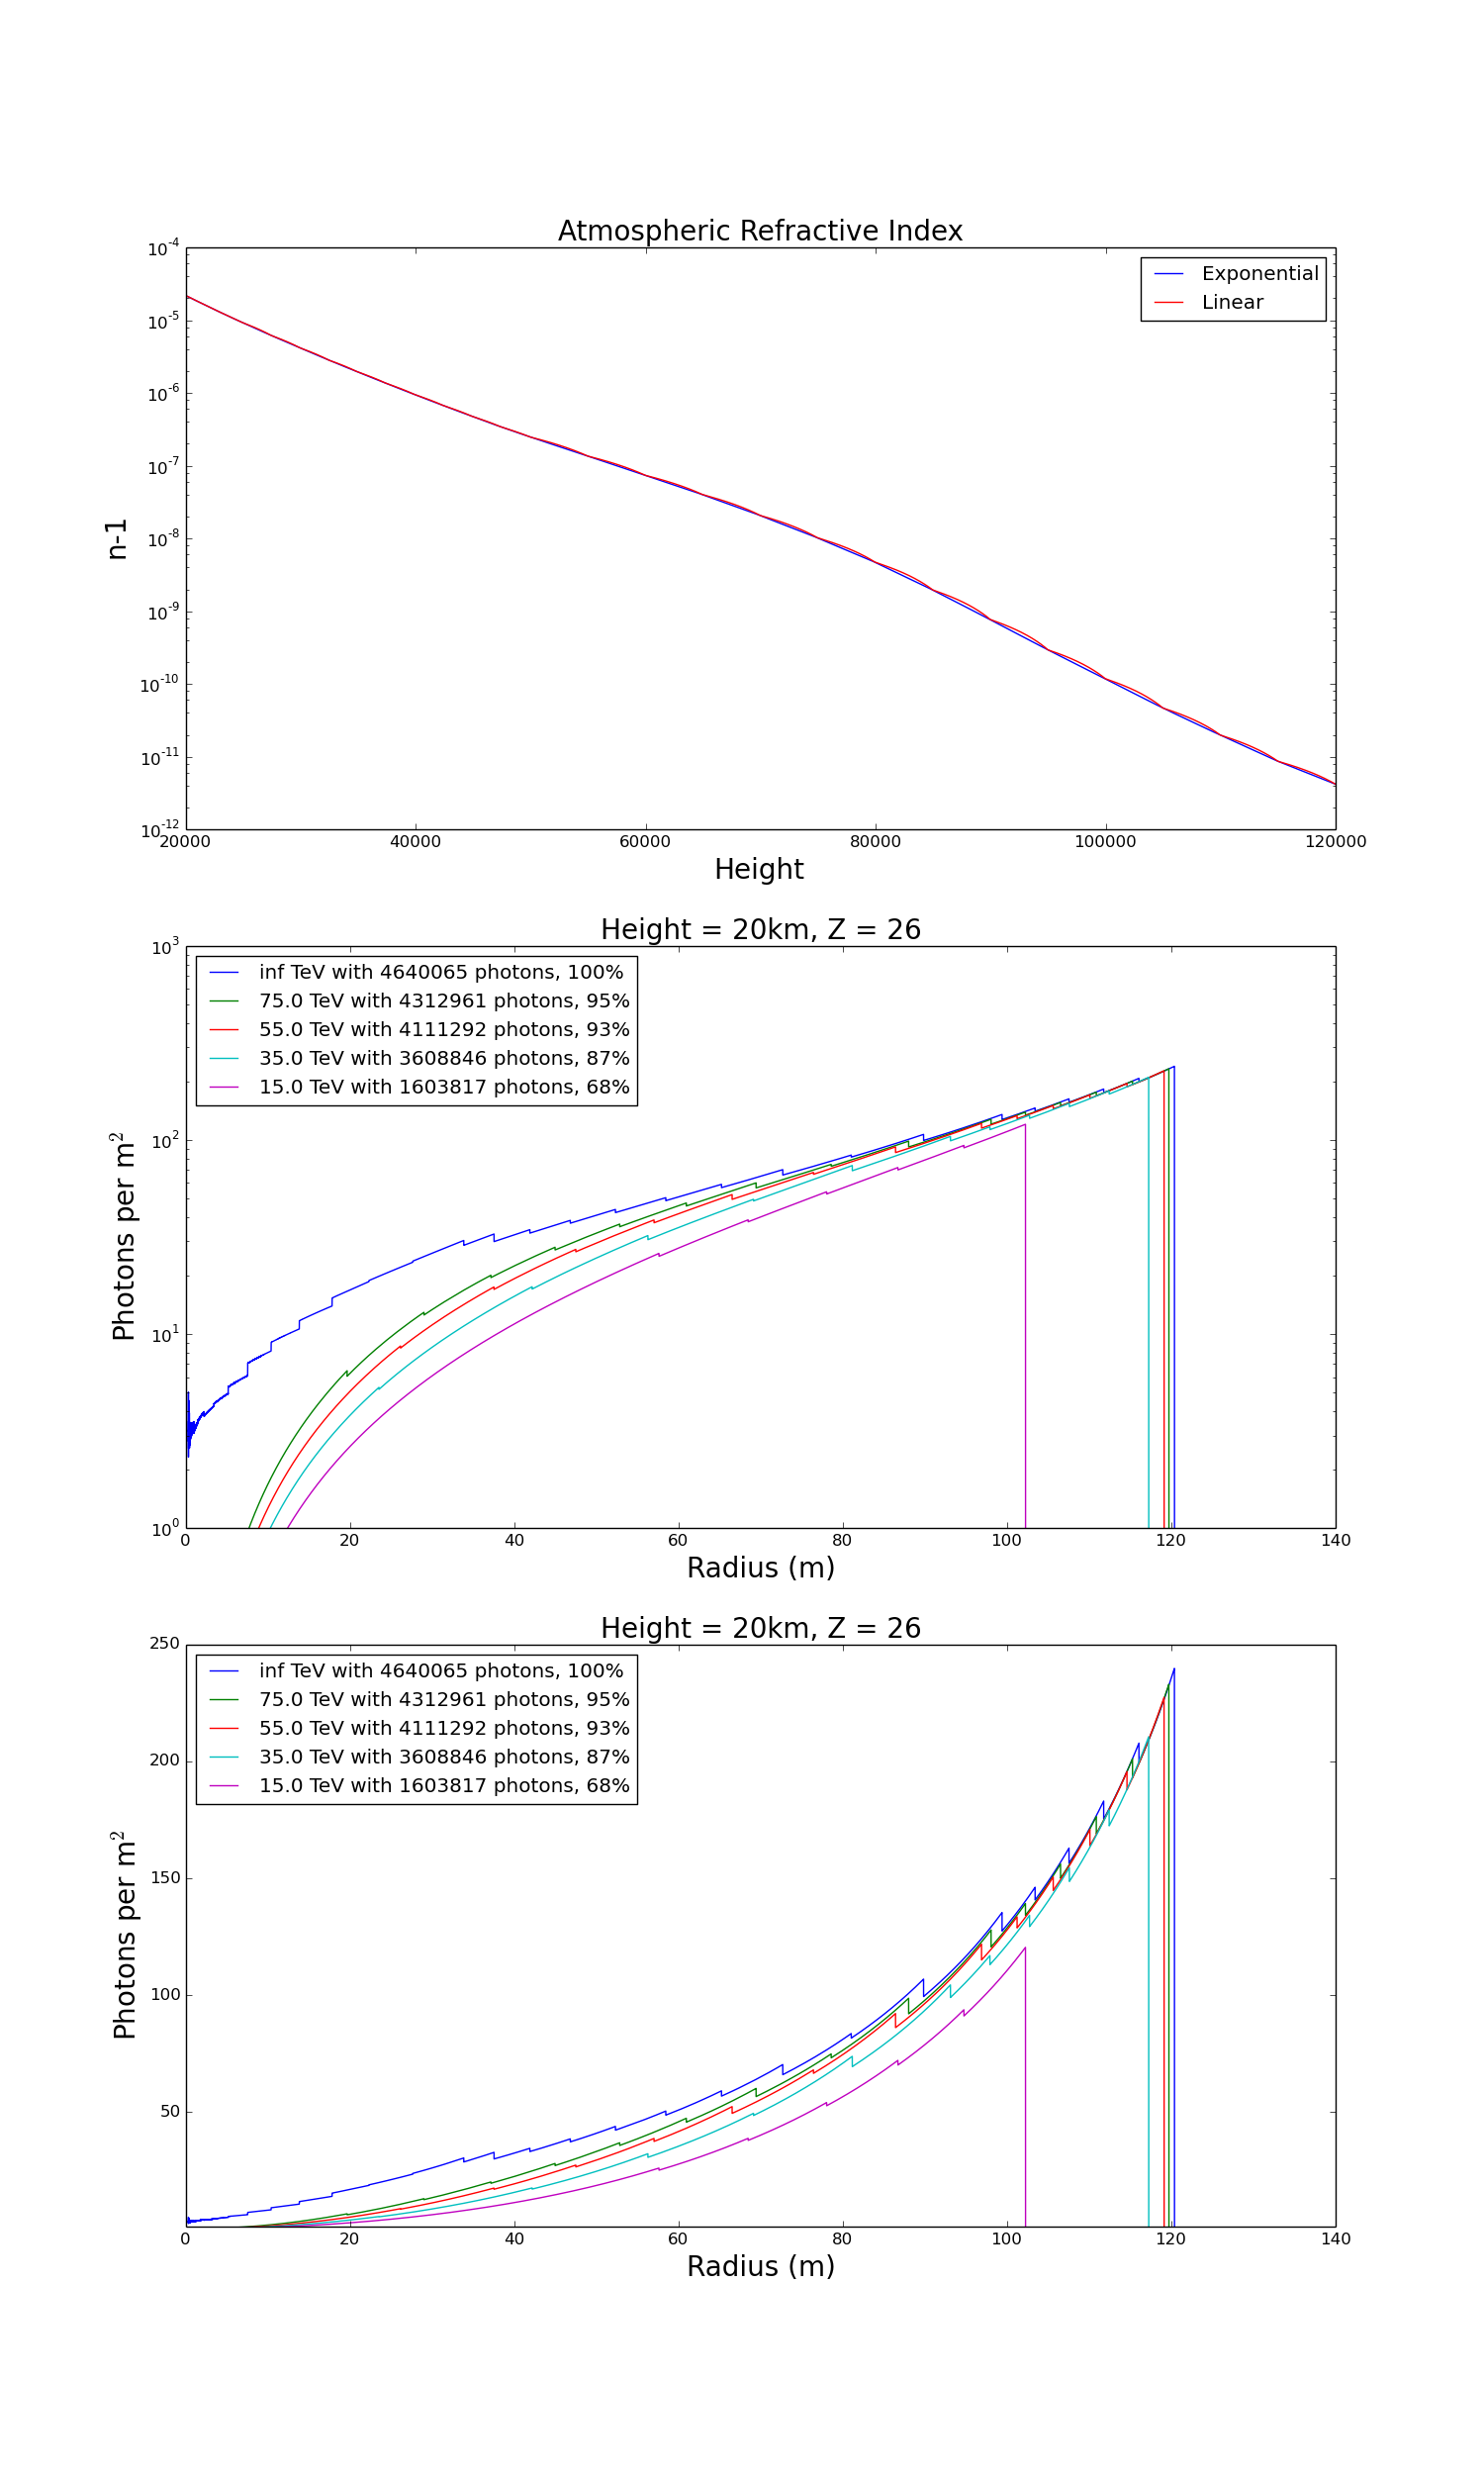
\includegraphics[height=0.9\textheight]{simulatedlpd}
\caption{The LPD obtained from simulation of an Iron Nucleus up to a first interaction height of 25km for a range of Core Energies. An altitude of 1.8km for the experimental array is assumed. Atmospheric absorption, although neglected, is broadly constant across the emission range leading to uniform amplitude scaling.}
\label{fig:lpd}
\end{center}
\end{figure}

The Refractive Index of the atmosphere, and thus the Cherenkov angle $\theta_{C}$, increases as the altitude decreases. The refractive index at a series of heights, based on data from the HESS site, is shown \ref{fig:lpd}. Exponentials are fitted between points to provide interpolation, and a comparison can be made to a linear interpolation that is also plotted. Despite the exponential interpolation, discontinuities in the second derivative of the refractive index prevent the LPD from being smooth in the simulation. This is unimportant, because in reality the variation due to atmospheric conditions and random noise will smear out any discontinuities in the LDF.

Emission continues until the first interaction with the atmosphere, occurring at a randomly distributed height we call $h$. Then for a given Telescope Array altitude above sea level, simple trigonometry yields the radius of the LDF on the ground:
\[ Radius(height = altitude_{array}) = \tan [\theta_{C}(h)] \times (h - altitude_{array})\]

Thus the upper atmosphere emission contributes to the inner LDF, while the lower atmosphere emission contributes to the outer LDF. We can also see ground emission radius as a function of height in \ref{fig:generalenergy}. We find that the high-radius emission (occurring near the first interaction region) varies little between different high energies. We deem this to be \textquoteleft Saturated Emission\textquoteright.

To accurately quantify Saturated Emission, we can compare the photon density to the theoretical maximum photon density, corresponding to an infinite-energy particle with $\beta =1$. The illustrated maximum is useful as a reference, although because the atmosphere is not modelled beyond an altitude of 120km, the small-radius emission is not accurately simulated entirely correctly. However, real cosmic rays in the considered energy regime will all cross the emission threshold and begin emission at an altitude much lower than 120km, so can be considered accurately modelled. Absorption WAS/WAS NOT modelled.

However, in the 4 telescope height region, the Cherenkov Threshold Energy is $ E_{Threshold} \approx 0.35$ TeV per Nucleon as shown in \ref{fig:lpd}! The saturation in for these heights occurs roughly at 0.7 TeV per Nucleon or something...

\subsection{First Interaction Height}
Cosmic Rays survival in from the top of the atmosphere follows an exponential decay with the number of 'interaction lengths' passed. The interaction length is dependent on the interaction cross section, which increases with density. Thus the number of interaction lengths increases exponentially as height decreases. The resultant decays occur most often at a height of $h \approx 40 \pm 10$ km , as seen in \ref{fig:generalheight}.

\begin{figure}
\begin{center}
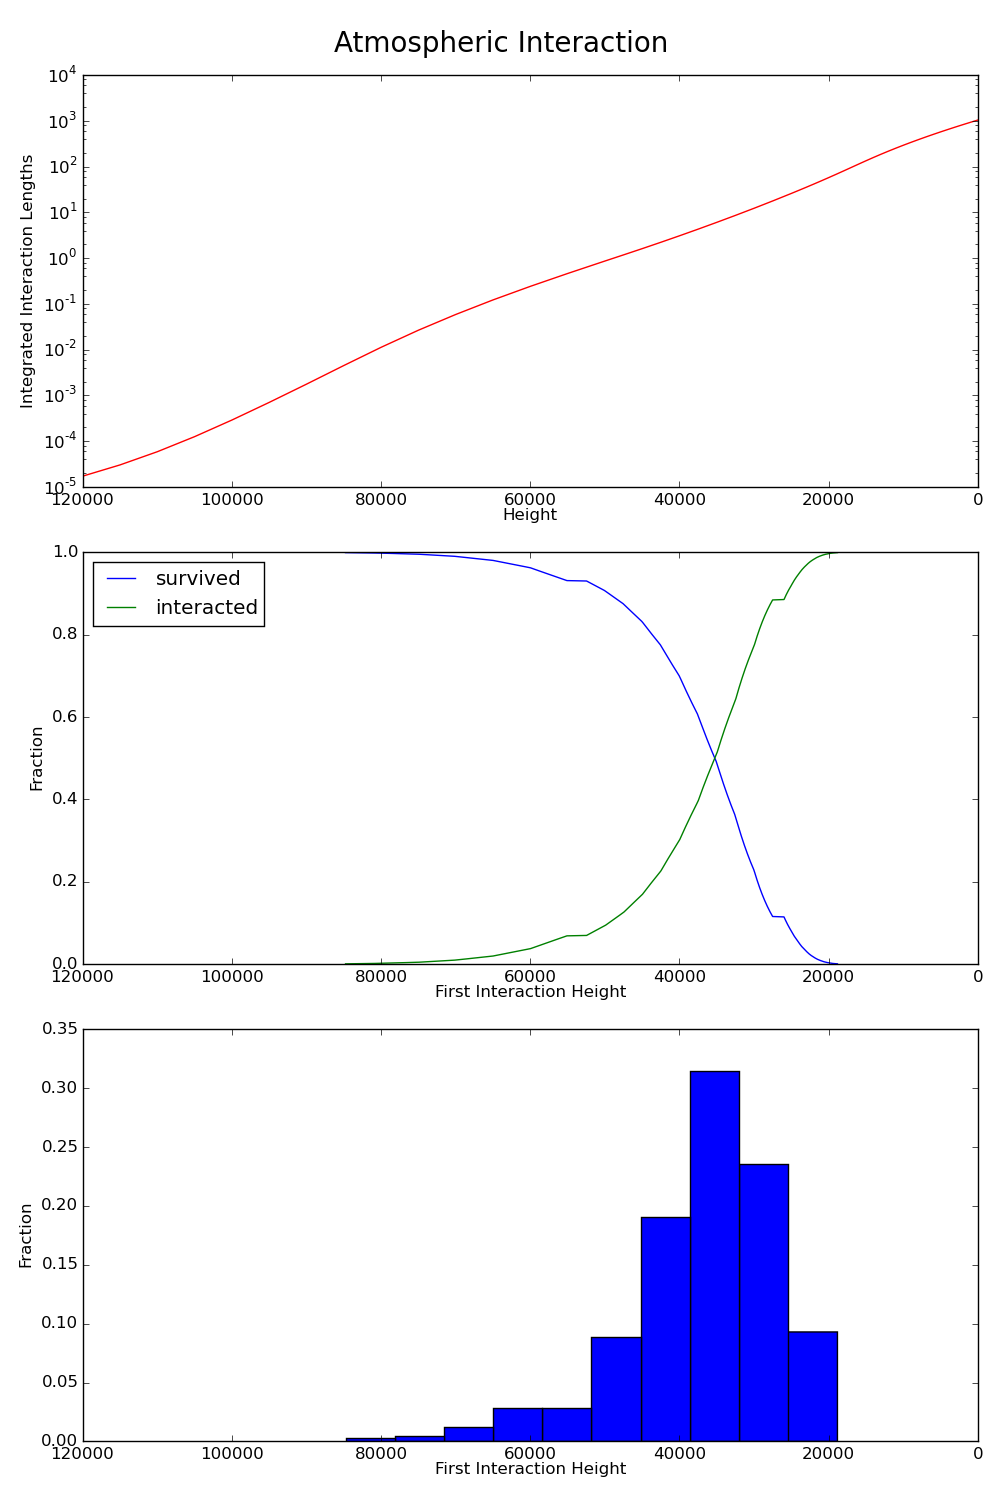
\includegraphics[height=0.9\textheight]{generalheight}
\caption{The integrated interaction lengths increases as height decreases. Thus the decay probability follows a exponentially increasing distribution. The mean first interaction height for all events is roughly 40km above sea level.}
\label{fig:generalheight}
\end{center}
\end{figure}

\subsection{Atmospheric Absorption}
The Cherenkov Light, mostly emitted in the visible blue part of the EM spectrum, experiences relatively little atmospheric absorption. The major of Rayleigh scattering-based atmospheric absorption occurs in the lower part of the troposphere, and thus the atmospheric absorption is almost independent of emission up to first interaction height.

\section{LPD Event Reconstruction}

\subsection{Log Likelihood Minimisation}
In order to fully reconstruct an event, we need to find the x/y core position, the Energy per Nucleon, the first interaction height and the charge. However, if one telescope in a five-telescope array does not observe DC light, this data point can be used to constrain the core position. Thus, for the LDF method to be applied, we require a minimum of five telescopes, four or more of which must image the DC light. We consider the amount of DC light that each telescope receives to be Poissonian \[  P_{i} ( N_{i, Received} \mid X, Y, Z, height, Epn )  =  \frac{ e^{- \lambda_{i} } \times \lambda_{i} ^{N_{i}} }{N_{i}!} \]

In order to reduce computing time, we can use Stirling's Approximation $\ln( N! )  \approx  N \ln(N) - N + \frac{1}{2} \ln(2 \pi N)$. Pure night sky background requires that there be more that X photons in a DC pixel, and for this Stirling's Approximation has an error of just Y?. We then minimise the Log Likelihood function \[ - \ln(L) = - \sum_{i=1}^{n} \ln(P_{i}) \approx  \sum_{i=1}^{n} [\lambda _{i} - N_{i} \ln(\lambda _{i}) + N_{i} \ln(N_{i}) - N_{i} + \frac{1}{2} \ln(2 \pi N_{i})]  \] where n is the total number of telescopes in the array.

\subsection{Extracting Charge Resolution}
Having reconstructed many events, we can then derive the $\sigma_{Z}$ of the dataset, giving us a number to directly compare the quality of event reconstruction. However, a simple Gaussian 68\% method will yield only half integer values of $\sigma_{Z}$ and very frequently 0. This will be unhelpful for comparisons of minor modifications of reconstruction methods.

Instead, we can assume a Gaussian with tails at the highest and lowest reconstructed charge values in the dataset. The size of the dataset can be used to calculate the fraction of events that the extreme values represent, and this probability can be converted into a \textquoteleft number of standard deviations from mean'. Dividing the Gaussian total width by the number of standard deviations gives us a value for $\sigma$. Although this will in most cases tend to overestimate the spread of the data, it will also be sensitive to all increases in the proportion of correctly reconstructed events.

\subsection{Iterative Scanning Minimisation}
Through $\sigma_{Z}$ calculation, we find that the LDF method initially provides very poor charge reconstruction. This is as a result of varying Threshold Energies and the sharp drop in the LDF above the maximum radius, which means the Log Likelihood is frequently discontinuous within the parameter space. Consequently, a Minuit-type minimisation algorithm will only be able to find a local minimum near the starting values for the fit parameters.

To overcome this problem, we can iterate over a series of starting values for the parameters, with the aim of scanning the true minimum among the many minima found. To simplify matters, we can scan only the integer Z values over the range $ 20 \leq Z \leq 32 $, rather than considering the charge to be a free floating parameter.

In order to reduce the number of calculations needed, we can consider the core position region derived from camera images, as in Hillas Analysis. Each telescope will have a Gaussian smeared central axis indicating the direction of the core. We overlay the simulated telescope array with a grid of points with grid width 1m. Then we select all points satisfy the condition of lying within the shower axis direction confidence interval for every telescope. The angular width of the confidence interval from the shower axis will be determined by the precision of the telescopes.

Having determined the relevant Height and Energy ranges, we can then consider combinations of Energy and Height for which the Energy is above the Cherenkov Emission Threshold (and is saturated!). This gives us a second set of starting \textquoteleft Coordinates \textquoteright.

The Z value is fixed and the LL function is then minimised with the assigned starting values, with the other four variables allowed to float freely. Minimisation typically scans 13 Z values, 10 core position coordinates, and 50 Height/Energy coordinates, yielding $ 13 \times 10 \times 50 = 6500$ minimisations in total. Such a technique is resource intensive but reduces $\sigma_{Z}$ by a factor of 5 or more. (CHECK this quantitatively and get a graph yo. Want to see some plateauing of sigma Z!).

\subsection{Boosted Decision Trees}
Using one quarter of a large sample of Monte Carlo data, we can train a Boosted Decision Tree (BDT) for a given telescope multiplicity, using the reconstructed x/y core position, height and energy, as well as the Log Likelihood. The BDT is told whether each event is \textquoteleft signal' (correctly reconstructed) or \textquoteleft background' (incorrectly reconstructed). 

For every simulated event, this trained BDT can then be used to assign a \textquoteleft Signal Probability'. On a second quarter of the dataset we can optimise a cut on the minimum signal probability, in order to maximise the ratio of signal to background. We find that the $\sigma_{Z}$ of the remaining \textquoteleft Test' Monte Carlo data is reduced when the same BDT cut is applied.

\section{HESS-type Event Reconstruction}
With a simulation of the HESS Cherenkov 5-Telescope Array we can verify the effectiveness of the technique. 
\subsection{First Interaction and Energy Saturation}
The mean first interaction height for all Cherenkov Emitting Cosmic Rays in the atmosphere is 40km, and neglecting variations in atmospheric density profiles around the Earth, this can be considered independent of experimental array. However, the multiplicity of event is determined by equipment efficiencies, altitude and telescope layout. When the HESS layout is simulated, we find that the 4 telescope events have a mean height of $h \approx 23 \pm 5$ km, as shown in \ref{fig:Hessheight}.

\begin{figure}
\begin{center}
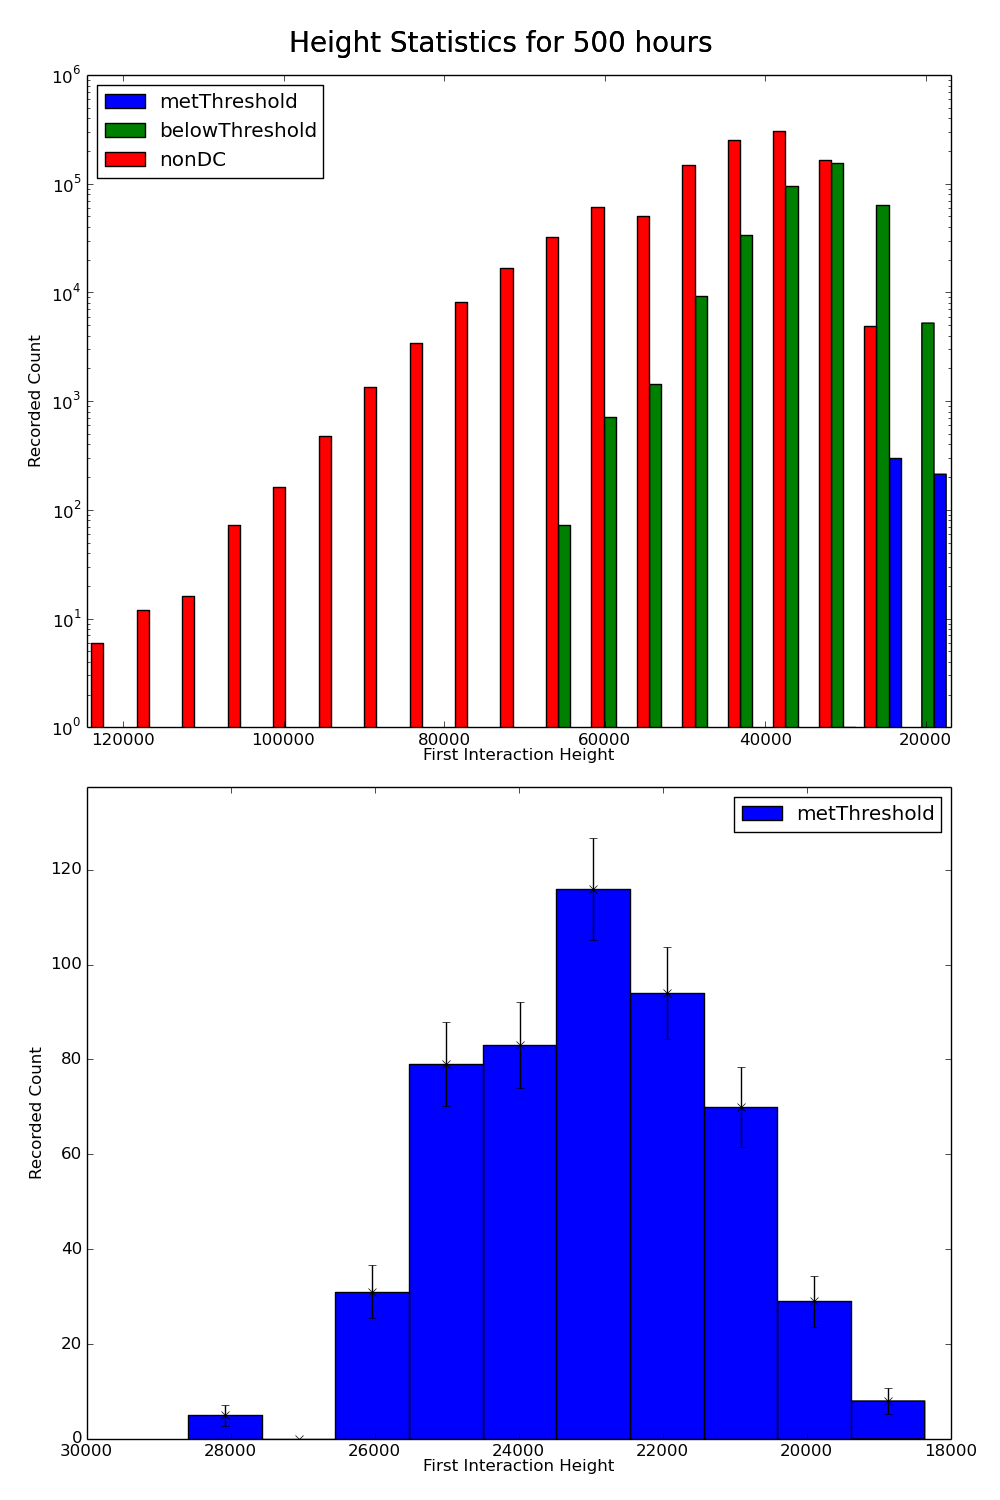
\includegraphics[height=0.9\textheight]{hessheight}
\caption{The mean first interaction height for all Cherenkov Events is 40km???. The mean first interaction height for 4 telescope events in the HESS array is 23km}
\label{fig:Hessheight}
\end{center}
\end{figure}

\subsection{Extended Air Shower Background}
A typical HESS image is shown in \ref{fig:hess}, with the DC pixel visible. For HESS cameras, the Extended Air Shower (EAS) produced after the first interaction of the Cosmic Ray overlaps the DC pixel and thus provides background in the LDF. As the Energy of the Cosmic Ray increases, the EAS speads over a larger angular area, and at smaller radii, the EAS-DC-shower direction axis contracts, leading to more overlap. Thus the background in the DC pixel increases with decreasing radius and increasing Energy. In addition, we have a fixed night sky background with 7 photons $m^{-2}$. We thus parameterise the background with \[ \rho_{bkg}  = 7 + 5E\]. The modeled background LPD is shown as part of REF. It begins to dominate above roughly 1 TeV per Nucleon, particularly in the case of smaller radii. 

\begin{figure}
\begin{center}
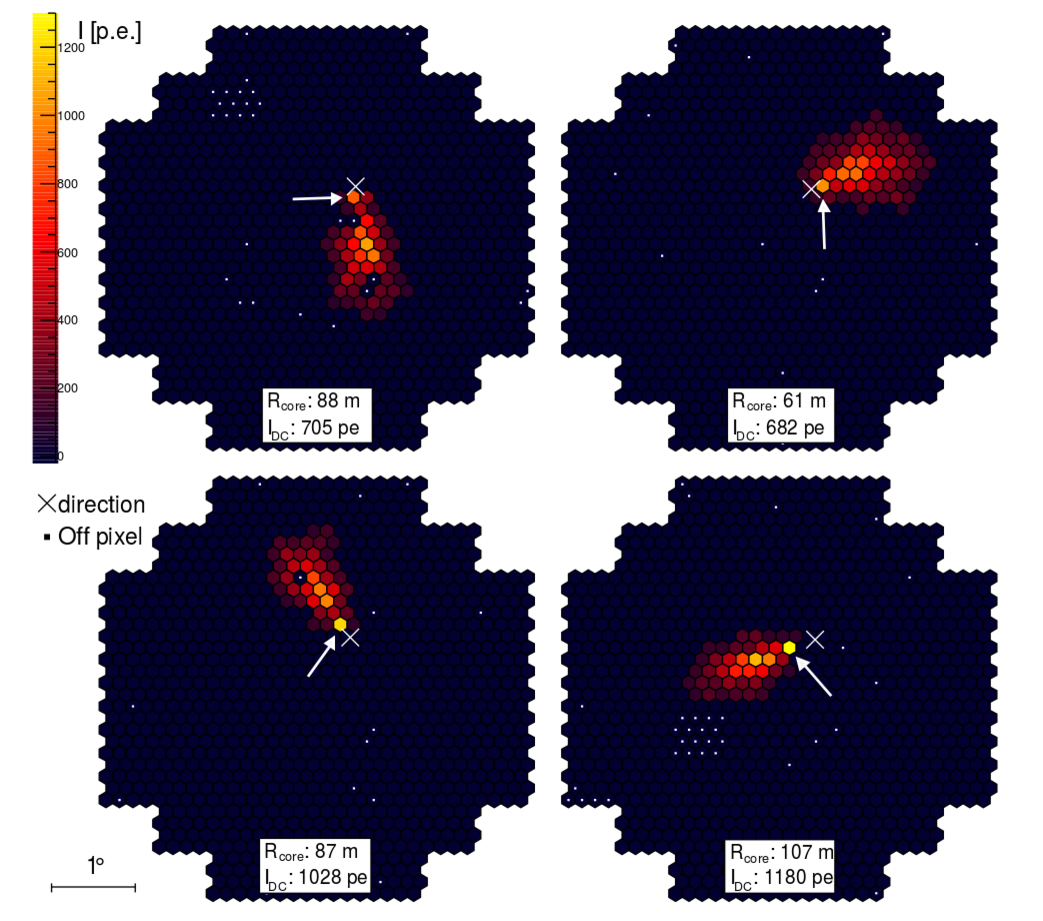
\includegraphics[width=0.9\textwidth]{hess}
\caption{A 4-camera HESS event. The shower direction is marked with a white cross, and the DC pixel is indicated with a white arrow. The shower axis passes through the shower direction, the DC pixel, and the center of the Extensive Air Shower region lying beyond the DC pixel.}
\label{fig:hess}
\end{center}
\end{figure}

\subsection{Reconstructed Charge Resolution}
In the preliminary HESS simulation, it was found that the 4 telescope event reconstruction had a charge resolution of $\sigma_{Z} = 1.4$. However, requiring that the BDT signal probability satisfied $P > 0.81$ removed $75 \%$ of events, while reducing the Charge resolution to $\sigma_{Z} = 0.9$ . With this cut, core position resolution was $d \approx 1.4 m $. For 5 telescope events, it was found that the charge resolution was also $\sigma_{Z} = 1.4$. However, requiring that the signal probability satisfied $P > 0.05$ removed $53 \%$ of events, including all wrongly reconstructed ones. This placed an upper limit on the charge resolution of $\sigma_{Z} < 0.35$ . With this cut, core position resolution was $d \approx 0.8 m $.

However, the simulated number of hours for the data was 1200? hours, and comparisons with HESS data show just 12 4-telescope events rather than 600. Thus, although the technique is valid and effective for HESS, the count rate will limit the potential to conduct any statistical analysis from this experiment.

\section{Optimised Telescope Array}
NO Background!!!!!
\subsection{Count Rates}

In order to improve the count rate of high-multiplicity events, we can consider a 3x3 array of Cherenkov Telescopes, which we want to use for identifying Cosmic Ray Elements accurately. In \ref{fig:optmiselayout} we see that the \textquoteleft High Multiplicity Count Rate' of events observed by 4 or more telescopes falls with increasing grid separation. We can clearly see that the optimum grid spacing will likely lie in the 20-50m region to provide a reasonable count rate. Competing with this effect is the reliance of LDF reconstruction on sampling the entire lateral distribution. Thus the reconstruction quality will decrease as Grid Width decreases. Further study of $\sigma_{Z}$ in this region is required to determine the optimum layout (not necessarily be a grid) for event reconstruction. 

\begin{figure}
\begin{center}
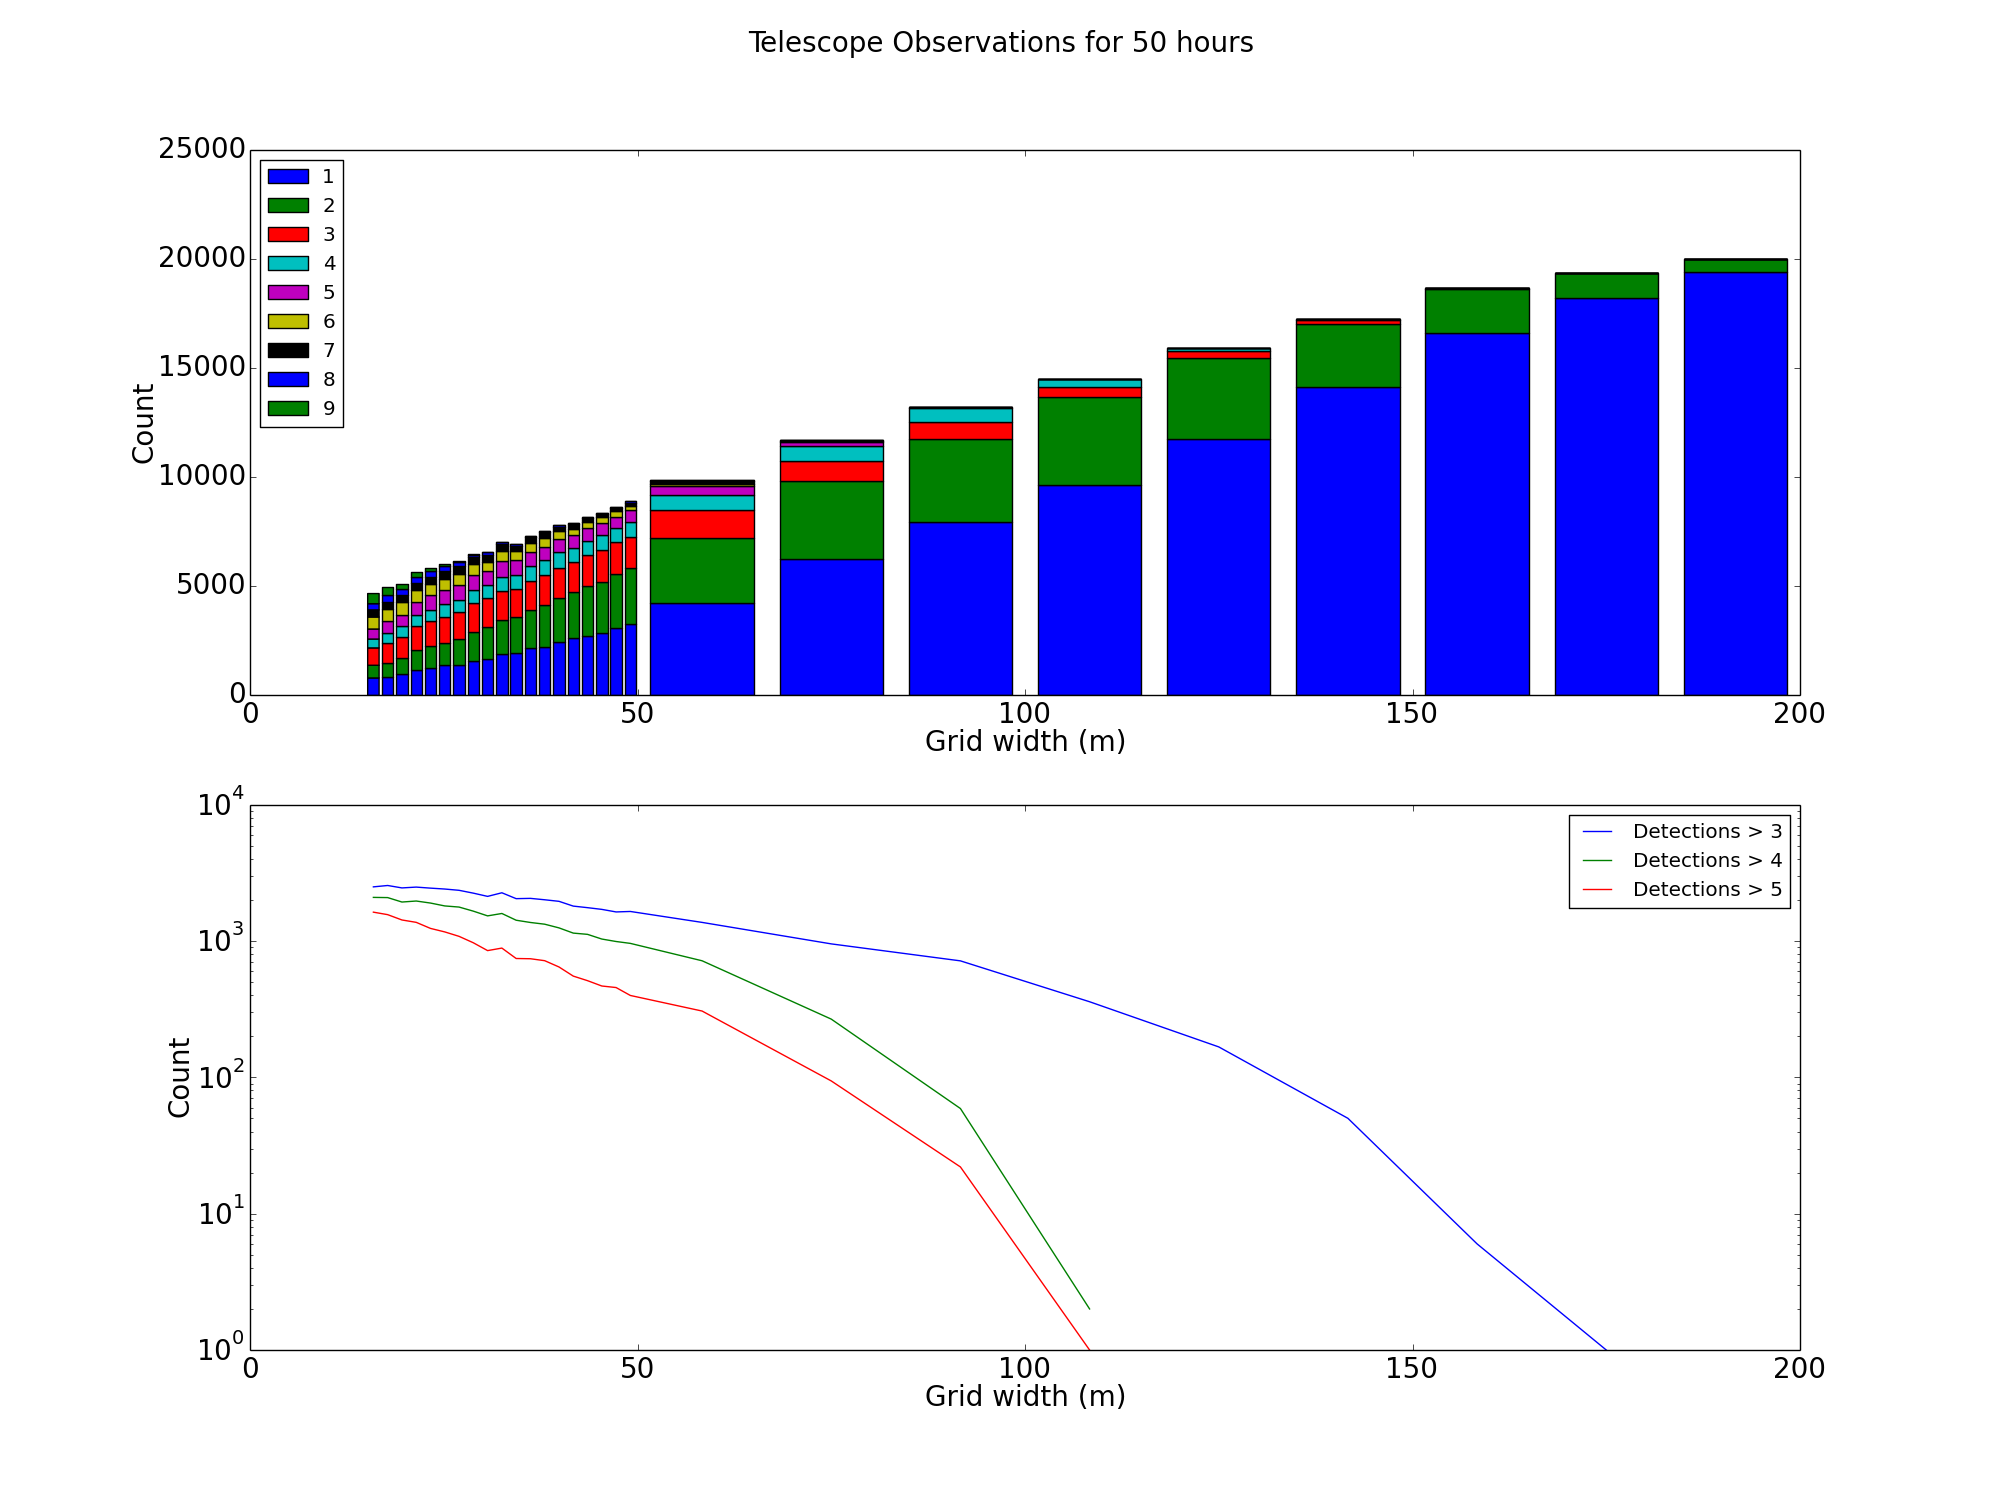
\includegraphics[width=0.9\textwidth]{optimiselayout}
\caption{A simulation of 50 hours of run time for various grid spacing for a 3x3 telescope array. Although raw count rate increases with increasing grid width, the \textquoteleft good count' rate of events observed by sufficient telescopes falls rapidly with increasing grid width}
\label{fig:optmiselayout}
\end{center}
\end{figure}

\subsection{Saturation Region Energies}

\subsection{High Speed Telescopes}
By definition, the EAS shower will arrive on the ground shortly before the DC light. There are currently several high-speed Cherenkov telescopes capable of distinguishing between these, allowing a background-free LDF to be fitted. Additional study of alternative energy regimes and layouts will also be considered for the case of a high-speed imaging telescope array. 

\section{Conclusion}
Preliminary results suggest that the LDF reconstruction technique will significantly improve charge reconstruction, to a level sufficient for cosmic ray abundance studies. However, reliance on high-multiplicity events means that although applicable to current experiments such as HESS, a new optimised telescope array would be required for a statistical analysis. Such an array may have a grid spacing of 20-50m, although further study is needed to determine the ideal layout.
\bibliographystyle{plain}
\bibliography{report}
\end{document}